\section{Three.js}
\setauthor{Romeo Bhuiyan}
\textbf{Three.js} is a JavaScript library that allows for the creation of interactive 3D graphics in the web 
browser. It is designed to work seamlessly with WebGL, which is a web-based 3D graphics API that allows 
developers to access the hardware-accelerated graphics capabilities of a user's computer. Three.js 
makes it possible to create rich 3D experiences with JavaScript and HTML, without the need for any plugins or downloads.
With Three.js, developers can create a wide variety of 3D scenes and animations, including but not limited to: 
realistic environments with dynamic lighting and shadows, complex 3D models and animations, interactive 3D 
games and simulations, and virtual reality (VR) and augmented reality (AR) experiences.
\\
\\
The library provides a large number of powerful features and abstractions that simplify 
the process of creating 3D graphics. It includes a number of built-in shapes, such as cubes, 
spheres, and cylinders, as well as more complex shapes that can be constructed from the 
vertices and faces of custom 3D models. Three.js also includes a number of materials that 
allow for realistic shading and texturing of 3D objects, as well as lights and cameras 
that can be positioned and manipulated to achieve the desired lighting and perspective effects.
Another important aspect of Three.js is its support for keyframe animations. This allows
 developers to animate objects over time, creating smooth transitions and movements. 
 The library also provides support for physics simulations, making it possible to 
 create complex and interactive 3D experiences that respond to user input.
\\
\\
\subsection{Three-vrm.js}
\setauthor{Romeo Bhuiyan}
\textbf{Three-vrm.js} is a JavaScript library that provides support for rendering 
and manipulating VRM (Virtual Reality Model) characters in web-based environments. 
It is built on top of Three.js, a widely-used library for creating 3D graphics and 
animations in web browsers.
Three-vrm.js offers a set of tools and APIs for working with VRM models, allowing 
developers to easily import, manipulate and animate VRM characters in their web-based 
projects. This includes support for importing VRM files, as well as manipulating and animating 
individual bones, rigging, morph targets, and materials of the characters as shown below in the figure \ref{fig:threevrmdebug}.
In addition to basic VRM functionality, three-vrm.js also includes a set of VRM-specific 
features and extensions. For example, it provides support for VRM's humanoids, which define 
the structure of a VRM character and allow for easy animation of the character. It also includes 
support for VRM's blend shapes, which are used to manipulate the shape of the character's 
face and expressions.
\\
\\
\begin{figure}[htb]
    \centering
    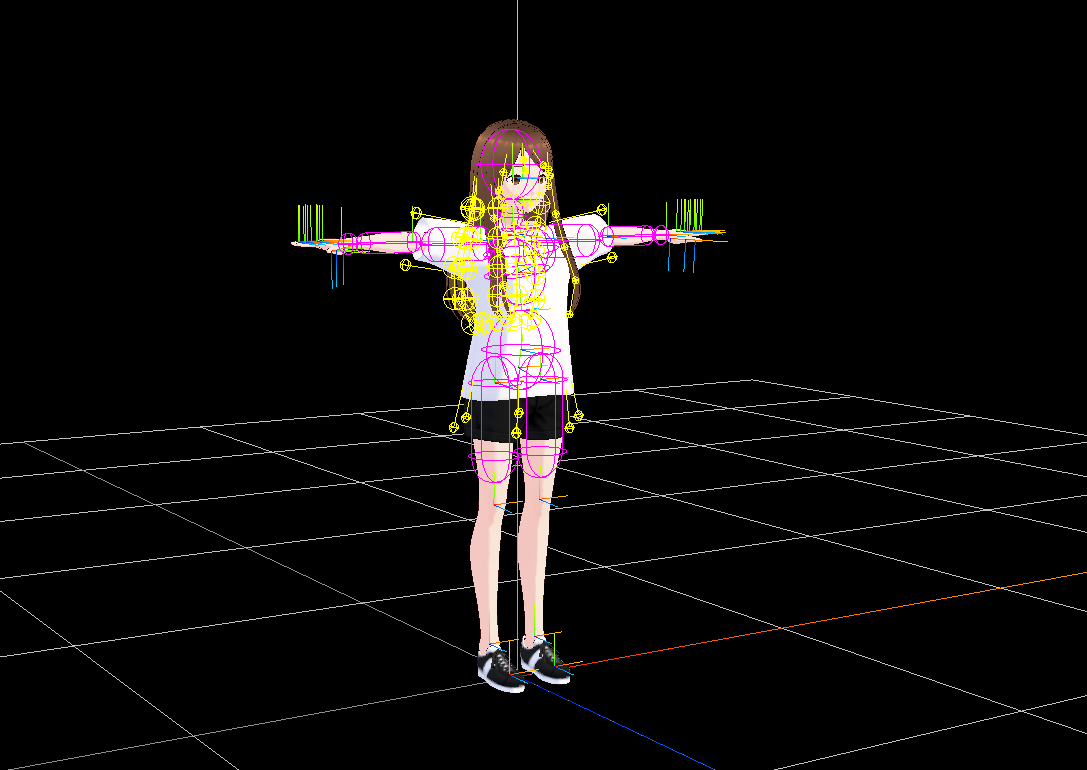
\includegraphics[width=0.9\textwidth]{pics/threevrmdebug.PNG}
    \caption{Three-vrm.js debug mode}
    \label{fig:threevrmdebug}
\end{figure}
\\
\\
\section{Decision between Webframeworks}
\setauthor{Christoph Lasinger}

\subsection{Angular}
\setauthor{Christoph Lasinger}
SPA stands for Single-Page application and is a type of web application that dynamically rewrites the 
current webpage instead of entirely reloading, i.e., requesting and displaying data from the server, it. 
The main benefits of an SPA are a more responsive user experience and avoiding the delay of having to wait 
for a website to load. Angular, the next version of the discontinued AngularJS, is a framework for such 
applications and is maintained and released by Google  in 2016.
\\
\\
Angular is a free and open-source project, meaning that the copyright owner, in this case the company Google,
gives anyone the right to distribute, modify and study the software for any purpose. Open-source software is 
however not the same as public-domain software as it still possesses a copyright, just a very open one, hence its name. 
One big advantage of such software over closed-source software is that anyone in the world can find bugs and make 
improvements for it, free of charge for the actual project-owner. Moreover, even if the publisher decides to no longer 
provide support and update their software, it can still be adapted and improved by its users. Amazingly, it can be seen 
in practise that this concept works and users really do improve open-source projects not only for their benefit but for 
that of others as well. For those reasons, Animotion too is an open-source project.\cite{Opensource}
%write more concretely about Angular
\\
\\
\subsection{React}
\setauthor{Christoph Lasinger}
Like Angular, React also is an open-source SPA-Framework, maintained and released by Meta (then Facebook) in 2013.
The easiest way to set up a React project is to use the officially supported command "create-react-app" 
(similar command for Next.js: create next-app) as it offers a modern build setup and is already preconfigured. 
Optionally, further parameters can be used to customize the project, for example "—template typescript" to use TypeScript 
instead of JavaScript. After the project is created, it can immediately be started and viewed on localhost using either 
"npm start" or "yarn start", depending on the package manager that is used. For development the command "npm run dev" is 
also very useful, as the website is immediately refreshed after saving any changes to the code. \cite{create-react}
% (is run dev also available to react or just nextjs?)
\\
\\
\subsection{Next.js}
\setauthor{Christoph Lasinger}
Hier werden noch Sachen eingefügt!
\\
\\
\subsection{Next.js}
\setauthor{Christoph Lasinger}
Sass stands for syntactically awesome style sheets and is a stylesheet language that compiles into CSS (Cascading Style Sheets). 
It extends CSS by quite a few features such as functions, variables, nested loops, mixins, etc. As a result, Sass enables 
stylesheets to be organized more easily and for design to be shared within and across projects. 
For example, instead of copying the hexadecimal value representing a colour for each and every element and possibly making mistakes, 
Sass makes it possible to store the colour code in a variable and access it using its more human-readable name.
Another useful feature of Sass not mentioned before is inheritance, an example of which can be seen in the following code snippet.
% insert sass code snippet here
Through the "extend" keyword CSS properties of one selector can be passed over to another selector which then automatically has those 
same properties set to the same values, thus inheriting them. In this example, legal-notice-text is merely a variant of the 
default-text and should therefore be in the same colour, font, and alignment. However, as legal-notice-text is of not much 
importance to the average user of the website, it should be rather small and take up little space. Because of the usage of 
inheritance, the code becomes more readable and easier to write and understand. \cite{SassInheritance}
\\
\\
\section{Object interaction with OrbitControls}
\author{Romeo Bhuiyan}
Orbit Controls
\\
\\
\section{Comparison of 3D rendering technologies}
\setauthor{Romeo Bhuiyan}
In order to display a virtual model on a canvas, a 3D rendering technology was required. Two libraries, 
GLTFLoader and WebGL, were evaluated using JavaScript to determine the best fit for the task at hand. 
The choice between the two ultimately depends on the specific needs and limitations of the project. 
Both GLTFLoader and WebGL are effective tools for rendering, but each have their own 
unique strengths and weaknesses.
\\
\\
\subsection{WebGL}
\setauthor{Romeo Bhuiyan}
\textbf{WebGL} is designed to work seamlessly with other web technologies such as HTML, CSS, and JavaScript, 
making it easy to integrate 3D graphics into web pages. It allows developers to create a wide range 
of interactive 3D applications and visualizations, including games, scientific 
simulations, data visualizations, and more.
One of the key features of WebGL is its ability to take full advantage of the GPU 
(graphics processing unit) on the user's device. This allows WebGL applications to 
run smoothly and efficiently, even on devices with limited resources. Additionally, WebGL provides 
a high level of compatibility across different browsers and devices, making it a widely accessible technology.
WebGL is supported by most modern web browsers, including Chrome, Firefox, Safari, and Edge. 
This means that developers can create WebGL applications that can be easily accessed by 
users on a wide range of devices and platforms.
\\
\\
\subsection{GLTFLoader}
\setauthor{Romeo Bhuiyan}
\textbf{GLTFLoader} is a JavaScript library that allows developers to load and parse 3D models in the GLTF 
(GL Transmission Format) file format. GLTF is a widely adopted file format for 3D models and is 
supported by many 3D modeling software, including Blender and SketchUp.
GLTFLoader provides a simple and easy-to-use API for loading and parsing GLTF models, 
which can then be displayed using WebGL. The library takes care of all the complex tasks 
involved in loading and parsing the model data, such as handling binary buffers, parsing 
JSON data and creating the geometry and materials for the model.
GLTFLoader also provides support for advanced features such as animations, skinning and morph 
targets, which are typically found in more complex 3D models. This allows developers to create 
more advanced and interactive 3D applications and visualizations.
One of the key benefits of using GLTFLoader is that it greatly simplifies the process of loading and 
displaying 3D models on the web. By using a standardized file format and a dedicated library, 
developers can focus on creating the logic and functionality of their application, rather than 
spending time on complex parsing and loading tasks.
Additionally, GLTF is a highly efficient format, which means that it can be loaded faster, 
and also the files are smaller in size, making it a great choice for loading 3D models on the web.
\\
\\
\subsection{Conclusion}
In conclusion, GLTFLoader is a powerful tool for creating 3D graphics for the web that 
offers several advantages over WebGL. One of the main benefits of using GLTFLoader is 
its ability to handle the loading and parsing of GLTF (GL Transmission Format) files, 
which are a widely-used format for 3D models. This eliminates the need for developers 
to write their own code to handle file loading and parsing, saving time and effort. 
Additionally, GLTFLoader provides a more streamlined and convenient way to work with 
3D models, as it allows developers to easily import and use pre-existing models rather 
than having to create them from scratch. Furthermore, GLTFLoader also supports various 
features such as animations, cameras, lights and many more which can be easily integrated 
with web pages. Therefore, it is more efficient and convenient for the purpose of Animotion 
to work with 3D models on the web, GLTFLoader is the best choice as seen below in the figure. \ref{fig:gltfloader}
\\
\\
\begin{figure}[htb]
    \centering
    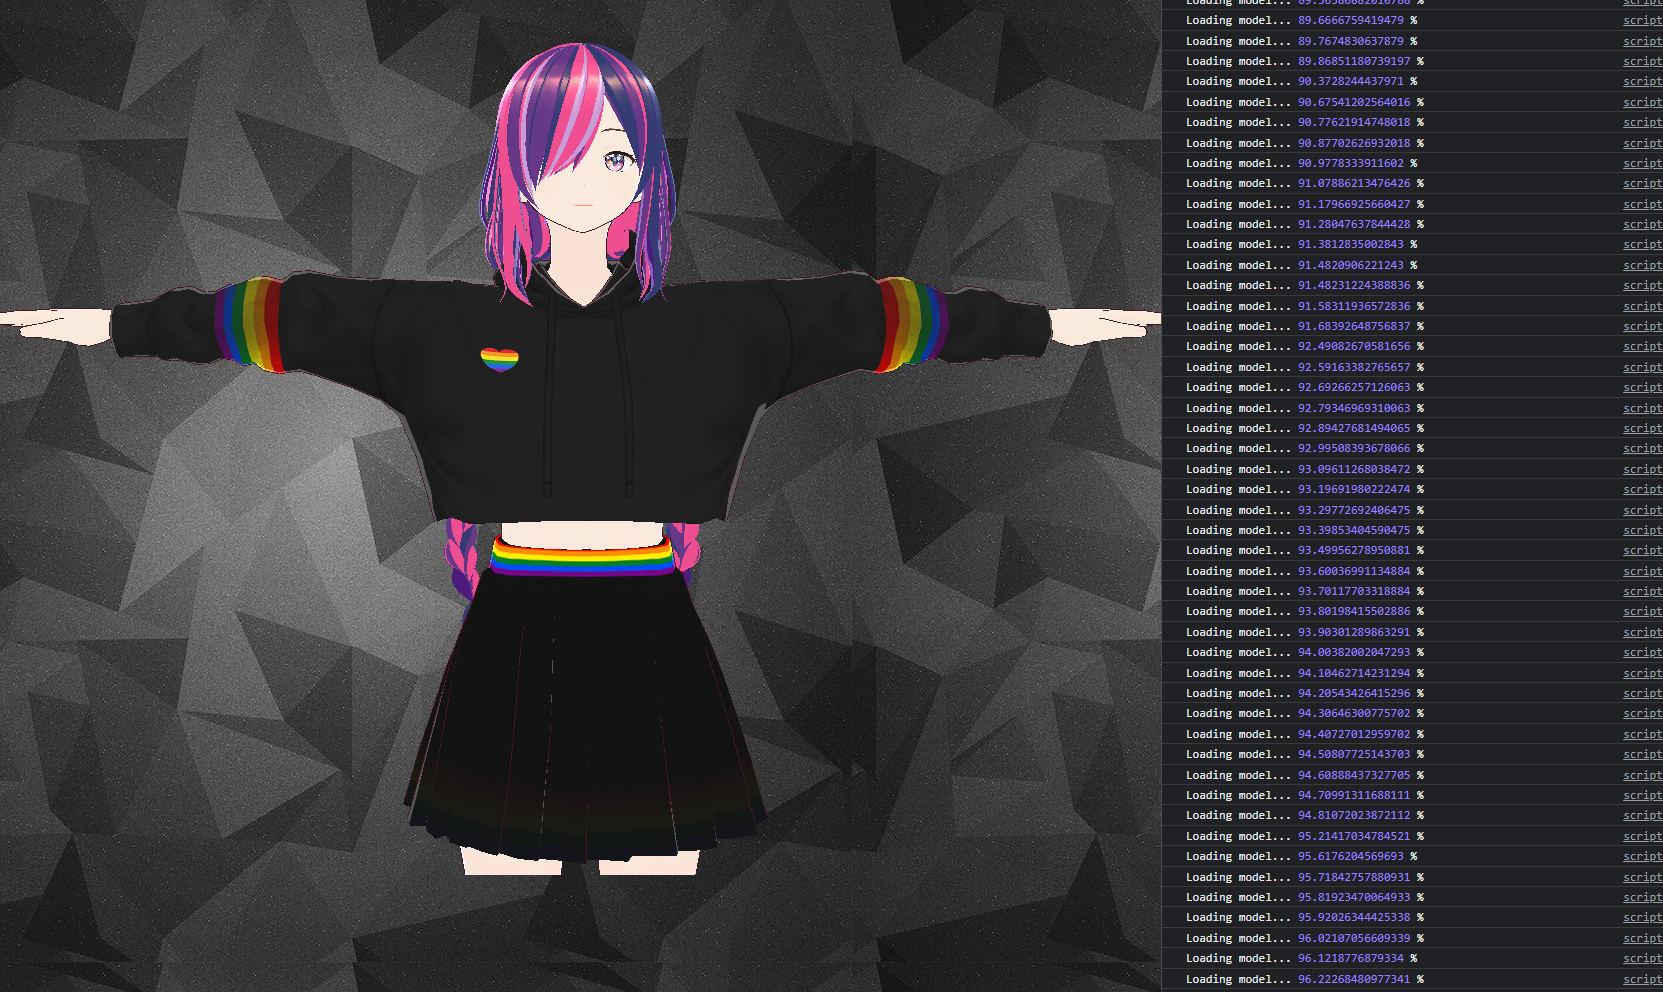
\includegraphics[width=0.9\textwidth]{pics/GLTFLoader.png}
    \caption{Loading the model with the help of GLTFLoader}
    \label{fig:gltfloader}
\end{figure}
\\
\\
\newpage
\section{Calculation of the virtual reality model} 
\setauthor{Romeo Bhuiyan}
Controlling a VRM on a website involves a complex process that involves 
capturing the user's inputs, updating the VRMs position and orientation in real-time, 
and rendering the updated model for display on the user's device.
The first step in this process is for the user to interact with the VR model 
using a device such as a VR headset or a mouse and keyboard. The inputs from the 
user are then captured by the website and sent to the server. The server then 
uses these inputs to update the VR model's position and orientation in real-time. 
\\
\\
Once the VR model has been updated, it is then rendered, and the new frame is 
sent back to the user's device for display. This process repeats as the user 
continues to interact with the VR model. 
To achieve this, various technologies are needed such as GLTFLoader\cite{GLTFLoader} from the THREE\cite{threejs}
libraries for rendering the VR model in the browser, WebSockets for real-time 
communication between the client and server, and a physics engine to simulate 
the movement and interactions of the VR model. 
\\
\\
\subsection{Blendshape}
\setauthor{Romeo Bhuiyan}
Blendshape is a technique used in 3D animation and computer graphics to create a smooth transition between different shapes or expressions of a 3D model. 
It works by creating a set of \emph{target} shapes for a 3D model, each representing a different expression or shape, 
and then using a set of weights or \emph{blend} values to interpolate between these target shapes, creating a 
smooth transition between them. This allows animators to create a wide range of expressive characters with a 
limited number of 3D models. Blendshapes are commonly used in animation, film and game industry.
\\
\\
\subsection{Lerp}
\setauthor{Romeo Bhuiyan}
The Lerp function, short for Linear Interpolation, is a mathematical function that is 
used to smoothly blend between two values. The function takes three arguments: a start value, 
an end value, and a weight. The weight is a value between 0 and 1 that represents the proportion 
of the blend between the start and end values.
For example, if the weight is set to 0, the function will return the start 
value, and if the weight is set to 1, the function will return the end value. 
If the weight is set to 0.5, the function will return the midpoint between the 
start and end values. By adjusting the weight, the Lerp function can be used to 
smoothly transition between any two values over time.
In the context of computer graphics, Lerp function is widely used for 
interpolating values such as position, rotation, and color, to make the 
animation smooth. It's also used in physics simulations, game development, 
and other fields where the smooth transition of values is needed.
\\
\\
\subsection{Determining mouth expressions}
\setauthor{Romeo Bhuiyan}

\begin{lstlisting}[language=Python,caption=Shape of mouth,label=lst:shapeOfMouth]
    for each shape in ["I", "A", "E", "O", "U"]
        Blendshape.setValue(PresetName[shape], 
        lerp(riggedFace.mouth.shape[shape], 
        Blendshape.getValue(PresetName[shape]), 0.5))

\end{lstlisting}
This pseudocode \ref{lst:shapeOfMouth} is a loop that iterates over an array containing the shapes \texttt{A, E, I, O, U}. 
The purpose of the loop is to blend the shape of a rigged face's mouth with a preset value of a 
Blendshape object for each of these shapes. The loop starts by setting the value of the Blendshape 
object to a blended value between the shape of the rigged face's mouth \texttt{(riggedFace.mouth.shape[shape])}
and the current value of the Blendshape object \texttt{(Blendshape.getValue(PresetName[shape]))}. 
The blend is done using the lerp function, which stands for linear interpolation. 
This function takes three arguments: the start value, the end value, and the weight of blending. 
In this case, the weight is set to 0.5, resulting in an even blend between the two values.
Once the blended value is calculated, it is set to the Blendshape object using the PresetName 
as the key. This process is repeated for each shape in the array, allowing the developer to 
easily blend the shape of the rigged face's mouth with preset values for multiple shapes.
\\
\\
\subsection{Blinking eyes}
\setauthor{Romeo Bhuiyan}
\begin{lstlisting}[language=Python,caption=Blinking of the eyes,label=lst:blinking]
    riggedFace.eye.l = lerp(clamp(1 - riggedFace.eye.l, 0, 1), Blendshape.getValue(PresetName.Blink), 0.5)
    riggedFace.eye.r = lerp(clamp(1 - riggedFace.eye.r, 0, 1), Blendshape.getValue(PresetName.Blink), 0.5)
    riggedFace.eye = Kalidokit.Face.stabilizeBlink(riggedFace.eye, riggedFace.head.y)
    Blendshape.setValue(PresetName.Blink, riggedFace.eye.l)

\end{lstlisting}
This pseudocode \ref{lst:blinking} is a code block that performs blinking animation on a VRM model. 
The code uses the Lerp function, the clamp function, and the stabilizeBlink function 
to animate the eyes of the rigged face.
\\
\\
The first two lines of the code use the Lerp function to blend the current value of the left and right eye shapes 
\texttt{(riggedFace.eye.l and riggedFace.eye.r)} with a preset Blink value from the Blendshape object. The Lerp 
function takes the clamp of the inversed eye shape values \texttt{(1 - riggedFace.eye.l and 1 - riggedFace.eye.r)}, 
which clamps the values to between 0 and 1, and the preset Blink value, which is obtained using \texttt{Blendshape.getValue(PresetName.Blink)}. 
The weight of the blend is set to 0.5, resulting in an even blend between the two values.
\\
\\
The third line of the code stabilizes the blinking animation of the eyes by calling 
the stabilizeBlink function from the \texttt{Kalidokit.Face} module. This function takes the 
current eye shape \texttt{(riggedFace.eye)} and the head's y position \texttt{(riggedFace.head.y)}  as arguments 
and returns a stabilized eye shape.
\\
\\
Finally, the fourth line of the code sets the Blink value of the Blendshape object to the 
stabilized left eye shape \texttt{(riggedFace.eye.l)}. This will result in a smooth and stable blinking  
of the eyes on the VRM model.
\\
\\
In summary, this pseudocode is a code block that animates the eyes of a VRM model by 
blending the current eye shape with a preset Blink value, stabilizing the blinking animation, 
and updating the Blink value of the Blendshape object. The code uses the Lerp function, the clamp 
function, and the stabilizeBlink function to create a smooth and stable blinking animation on the VRM model.
\\
\\
\subsection{Positioning the model}
\setauthor{Romeo Bhuiyan}

\begin{lstlisting}[language=Python,caption=Position of the model,label=lst:position]
    function rigPosition(name, position={x:0, y:0, z:0}, dampener=1, lerpAmount=0.3) {
        if (currentVrm is not defined) {
          return;
        }
        Part = currentVrm.humanoid.getBoneNode(name from THREE.VRMSchema.HumanoidBoneName);
        if (Part is not defined) {
          return;
        }
        vector = new THREE.Vector3(position.x * dampener, position.y * dampener, position.z * dampener);
        Part.position.lerp(vector, lerpAmount);
    }
      
      oldLookTarget = new THREE.Euler();
      function rigFace(riggedFace) {
        if (currentVrm is not defined) {
          return;
        }
        rigRotation("Neck", riggedFace.head, 0.7);
      
        Blendshape = currentVrm.blendShapeProxy;
        PresetName = THREE.VRMSchema.BlendShapePresetName;
    }
      

\end{lstlisting}
This pseudocode \ref{lst:position} is a code block that positions a VRM model according to a set of defined parameters. 
The code block consists of two functions: rigPosition and rigFace.
\\
\\
The \textbf{rigPosition function} takes three arguments: name, position, dampener, and lerpAmount. The name argument is the name 
of the part of the VRM model that needs to be positioned, the position argument is an object with x, y, and z properties 
that represent the desired position of the part, the dampener argument scales the position values, and the lerpAmount 
argument is the weight of the blend between the current position and the desired position.
The function starts by checking if the currentVrm is defined, and if it's not, the function returns without executing further code. 
If currentVrm is defined, the code uses the \texttt{humanoid.getBoneNode} method to retrieve the part specified by the name argument. 
If the part is not defined, the function returns without executing further code.
If the part is defined, the code creates a new \texttt{THREE.Vector3} object with the desired position 
values (scaled by the dampener argument), and the Part.position property is blended towards the 
desired position using the lerp method. The weight of the blend is set by the lerpAmount argument.
\\
\\
The \textbf{rigFace function} takes one argument: riggedFace, which represents the face of the VRM model. The function starts 
by checking if the \emph{currentVrm} is defined and if it's not, the function returns without executing further code.
If \emph{currentVrm} is defined, the function calls the rigRotation method and passes two arguments: \emph{Neck} and \emph{riggedFace.head}, 
with a third optional argument of 0.7. This rotates the neck of the VRM model according to the head position.
The function also defines the Blendshape variable and assigns it to the \texttt{blendShapeProxy} property of the \emph{currentVrm} object. 
The \texttt{PresetName} variable is set to the \texttt{BlendShapePresetName} property from the \texttt{THREE.VRMSchema} object.
\\
\\
\subsection{Animating the body}
\setauthor{Romeo Bhuiyan}
\begin{lstlisting}[language=Python,caption=Animating the rest of the body,label=lst:restbody]
    if (pose2DLandmarks && pose3DLandmarks) {
    riggedPose = solvePose(pose3DLandmarks, pose2DLandmarks, "mediapipe", videoElement);
    rotate("Hips", riggedPose.Hips.rotation, 0.7);
    position("Hips", -riggedPose.Hips.position.x, riggedPose.Hips.position.y + 1, -riggedPose.Hips.position.z, 1, 0.07);

    rotate("Chest", riggedPose.Spine, 0.25, 0.3);
    rotate("Spine", riggedPose.Spine, 0.45, 0.3);

    rotate("RightUpperArm", riggedPose.RightUpperArm, 1, 0.3);
    rotate("RightLowerArm", riggedPose.RightLowerArm, 1, 0.3);
    rotate("LeftUpperArm", riggedPose.LeftUpperArm, 1, 0.3);
    rotate("LeftLowerArm", riggedPose.LeftLowerArm, 1, 0.3);

    rotate("LeftUpperLeg", riggedPose.LeftUpperLeg, 1, 0.3);
    rotate("LeftLowerLeg", riggedPose.LeftLowerLeg, 1, 0.3);
    rotate("RightUpperLeg", riggedPose.RightUpperLeg, 1, 0.3);
    rotate("RightLowerLeg", riggedPose.RightLowerLeg, 1, 0.3);
}

\end{lstlisting}
The pseudocode ,\ref{lst:restbody} you have posted describes an animation process for a VRM body. 
The code checks if the \emph{pose2DLandmarks} and \emph{pose3DLandmarks} are available. If they are both available, 
the code calculates the rigged pose using the function \texttt{solvePose} with the \emph{pose3DLandmarks}, \emph{pose2DLandmarks}, 
\emph{mediapipe}, and \emph{videoElement} as input parameters. The function \texttt{solvePose} returns the rigged pose, which 
is then stored in the variable \texttt{riggedPose}.
The code then rotates and positions various body parts of the VRM model based on the values obtained from the 
rigged pose. For example, the hips are rotated based on the value of \texttt{riggedPose.Hips.rotation} with a weight 
of 0.7, and their position is changed to \texttt{x: -riggedPose.Hips.position.x, y: riggedPose.Hips.position.y + 1, z: 
-riggedPose.Hips.position.z} with a weight of 1 and a smoothing factor of 0.07. Similar operations are performed 
for the chest, spine, arms, and legs.
The rotation and position of each body part is performed using two separate functions: \texttt{rotate} and 
\texttt{position}. The first parameter of each function specifies the name of the body part to be animated, 
while the remaining parameters specify the values used for rotation or position, weight, and smoothing factor.
In this way, the VRM model's body is animated according to the solved pose information.
\\
\\
\subsection{Animation of both hands}
\setauthor{Romeo Bhuiyan}
\begin{lstlisting}[language=Python,caption=Animating the left hand,label=lst:hands]
    if (leftHandLandmarks) {
        # Obtain the rotation information of the left hand
        riggedLeftHand = Hand.solve(leftHandLandmarks, "Left");
      
        # Apply the rotation to the left hand rig
        rigRotation("LeftHand", {
          z: riggedLeftHand.LeftWrist.z,
          y: riggedLeftHand.LeftWrist.y,
          x: riggedLeftHand.LeftWrist.x,
        });
      
        # Apply the rotation to each of the finger bones
        rigRotation("LeftRingProximal", riggedLeftHand.LeftRingProximal);
        rigRotation("LeftRingIntermediate", riggedLeftHand.LeftRingIntermediate);
        rigRotation("LeftRingDistal", riggedLeftHand.LeftRingDistal);
        rigRotation("LeftIndexProximal", riggedLeftHand.LeftIndexProximal);
        rigRotation("LeftIndexIntermediate", riggedLeftHand.LeftIndexIntermediate);
        rigRotation("LeftIndexDistal", riggedLeftHand.LeftIndexDistal);
      }
\end{lstlisting}
The provided pseudocode \ref{lst:hands} animates the left (same for the right) hand of a VRM character. 
It starts by checking if the left hand landmarks have been detected. 
If they have, the code then calculates the rotations of the left hand by 
using the \texttt{Hand.solve} function, which takes in the left hand landmarks and the string \texttt{Left}.
The resulting rotations are then applied to the left hand rig and each of the finger 
bones using the \texttt{rigRotation} function. For the left hand rig, the function is called with 
the string \texttt{LeftHand} and the rotation values for the x, y, and z axes, obtained from the 
\texttt{riggedLeftHand} object.
Similarly, the rotations of each finger bone are applied by calling the \texttt{rigRotation} function 
with the names of the bones, such as \texttt{LeftRingProximal},\texttt{LeftRingIntermediate}, and \texttt{LeftRingDistal}, 
and the corresponding rotation values obtained from the \texttt{riggedLeftHand} object. The same process is 
repeated for each of the other finger bones.